\section{Engine}

\subsection{Overview}

brief {}``what is engine'', honda cbr, etc.

maximise power output (performance application)

torque power curve, etc.

\subsection{ECU}

A specialized third-party component called the \emph{Engine Control Unit} (ECU) controls the fuel injector and spark coil systems that in turn control the combustion cycle of the engine. The particular model of ECU used by the Formula SAE car is the S80Pro from DTAFast \cite{s80pro}. The ECU uses the O$_{2}$, MAP, cam position, and crank position sensors to adjust the fuel injector and spark coil timings. This keeps the engine running smoothly. The ECU features a traction control system that monitors wheel slip and cuts spark and fuel to provide traction when one of the wheels is slipping. The ECU also collects the various sensor readings and makes them available to other electronic devices at a fixed frequency through a shared data bus. 

\begin{figure}[H]
\centering
%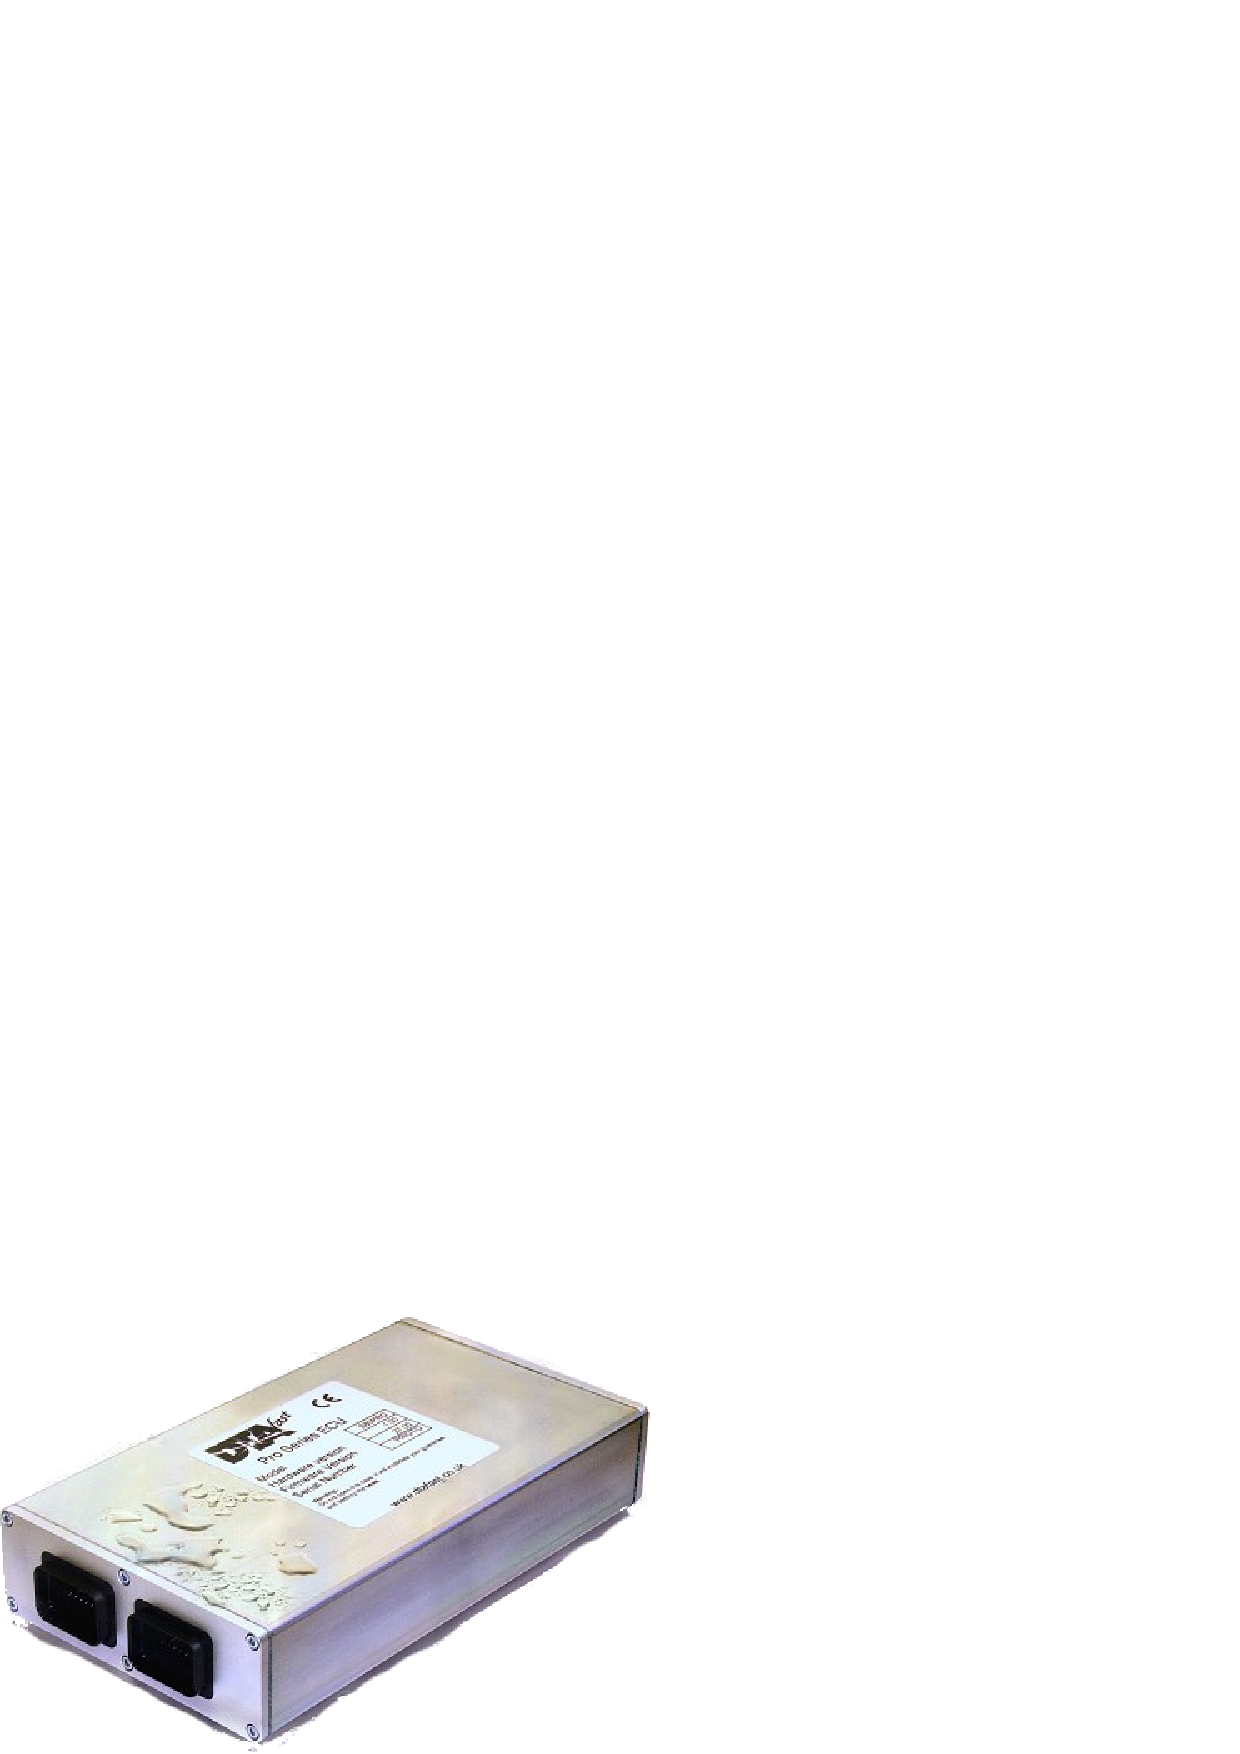
\includegraphics[scale=0.5]{Figures/s80.png}
\caption{The DTAFast S80Pro engine control unit.}
\label{fig:s80pro_product}
\end{figure}

\subsubsection{ECU Data interfaces\label{sec:background_ecu_data_interfaces}}

The ECU provides 3 digital communication methods:
\begin{itemize}
  \item An RS-232 link is used by the software that DTA provides for tuning and controlling the ECU. The serial protocol that the software uses is proprietary and undocumented.
  \item A read-only CAN bus interface that emits ECU data at a fixed frequency. The message format for the CAN data is documented in Appendix \ref{cha:ecu_can_spec}.
  \item Several CMOS-level discrete inputs:
  \begin{itemize}
    \item Launch Control toggle, which toggles the launch control feature in the ECU,
    \item Shift cut, which signals the ECU to reduce engine power before a downshift
    \item Traction control toggle, which toggles the traction control feature in the ECU,
    \item Traction control wet/dry, which switches between two different sets of traction control parameters in the ECU.
  \end{itemize}
\end{itemize}

Detailed descriptions of the ECU's launch control, shift cut, and traction control features can be found in the manual \cite{s80pro}.
 
\nomenclature{RS-232}{Recommended Standard 232, a byte-oriented serial communications protocol, typically asynchronous.}

\subsection{Intake and Exhaust}

Intake background, pressure waves, etc. Torque curve depends on length, 

\subsection{Research and Modelling of Variable Length Intake}

present research done by others on team, quantified runner length
dependence

intake length changes power

quantified length versus power on actual vehicle

chose optimal intake length

proposed variable length intake system for future work

\subsection{Starting System}

current requirements, starter motor, etc.

